\documentclass[10pt,a4paper]{article}
\usepackage[utf8]{inputenc}
\usepackage{amsmath}
\usepackage{amsfonts}
\usepackage{amssymb}
\usepackage{graphicx}
\begin{document}
\section{Zustandsdiagramme}
\begin{itemize}
\item In einem Zustandsdiagramm werden Zustandsgrößen gegeneinader aufgetragen um so die Änderung der Zustandsgrößen bei einem Prozess zu verdeutlichen.
\item Verändert man in einem System eine Zustandsgröße so ändern sich auch eine oder mehrere andere.
\subsection{Arbeitsprozesse mit idealen Gasen}
\item Der Zustand eines Gases wird durch die Zustandsgrößen p, T und V beschrieben. \newline 
\begin{figure}[hbtp]
\centering
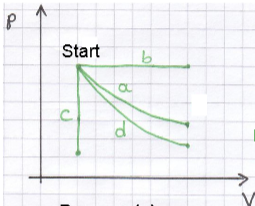
\includegraphics[scale=0.7]{zustandsdiagramm.PNG}
\end{figure}

\subsubsection{(a) Isothermer Prozess: T=const.}
\begin{equation}
W= \nu R T ln(\frac{V_2}{V_1})
\end{equation}
\subsubsection{(b) Isobarer Prozess p=const.}
\item Bei diesem Prozess wird der Druck des Mediums konstant gehalten.
\begin{equation}
W=p \Delta V
\end{equation}
\subsubsection{(c) Isochorer Prozess V=const.}
\item Bei diesem Prozess wird das Volumen des Mediums konstant gehalten.
\begin{equation}
W= \int^{V_2}_{V_1} p dV=0
\end{equation}
\subsubsection{(d) Adiabater Prozess}
\item Bei diesem Prozess findet kein Wärmeaustausch statt($\Delta Q=0$ ;$\Delta U=-W)$
\begin{align}
\gamma &= \frac{C_p}{C_V} \\
pV^\gamma &= konst. \\
TV^{\gamma-1}&=konst.
\end{align}
\subsubsection {Carnot-Prozess}
\item isotherme Expansion - adiabatische Expansion - isothereme Kompression - adiabatische Kompression
\begin{align}
\eta_{carnot} =\frac{T_0-T_u}{T_0} \\
f_{carnot} = \frac{T_u}{T_0-T_u}
\end{align}
\end{itemize}
\end{document}